
\clearpage\section{スクレイピングで取得した情報を習った技術と組み合わせる}
これまでの例で、ウェブページをスクレイピングして、必要な情報を取り出す方法を学びました。
次は、スクレイピングを習った技術と組み合わせることを学びます。
スクレイピングだけでも、かなりできることは広がりますが、やはりセンサーボードやJulius、OpenJtalkなど習った技術と組み合わせるとさらに便利で楽しいものが作れます。

\refstepcounter{Exercise}
\clearpage\section{\theExercise スクレイピングした情報をもとにセンサーを使う}
\addtocounter{Exercise}{-1}\refstepcounter{Exercise}\label{E:amedasSensor}
スクレイピングで得た情報を習った技術(センサーボードの使い方、OpenJtalk,
Juliusなど)と組み合わせて便利なことや楽しいことをする練習をしましょう。
この例では、アメダスのウェブページから取得した気温を使って暑いか\ruby{涼}{すず}しいかを判断してLEDで通知してくれるプログラムを試します。
その後にこのプログラムを変更して、気温以外の情報を使用してより高度な通知ができるようにしてみましょう。

まずは、実行してみましょう。

ターミナルを開いて、

hsed

と実行してスクリプトエディタを開きます

\begin{center}
  % Unhandled or unsupported graphics:
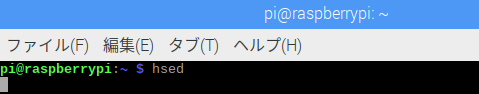
\includegraphics[width=\textwidth]{./text08-img/textbook-img013.png}

\end{center}
ファイル→
開く をクリックして\textbf{{\textasciitilde}/08/amedas\_led.hsp}を開きます。

\begin{center}
  % Unhandled or unsupported graphics:
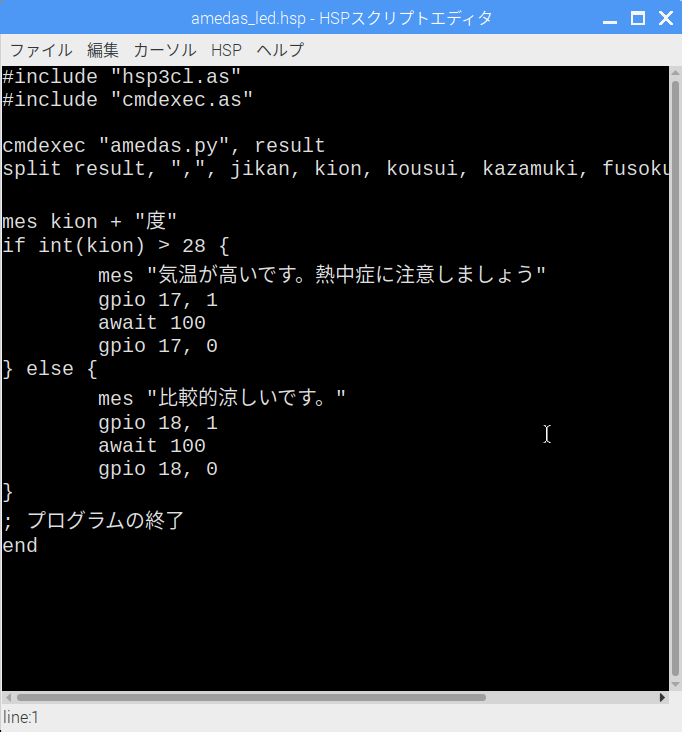
\includegraphics[width=12.173cm]{./text08-img/textbook-img038.png}

\end{center}

\bigskip


\bigskip

\clearpage
F5を押して実行してみましょう。



\begin{center}
  % Unhandled or unsupported graphics:
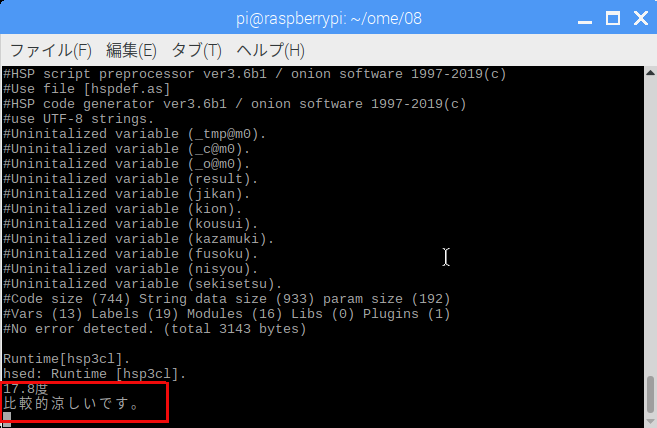
\includegraphics[width=\textwidth]{./text08-img/textbook-img039.png}

\end{center}
ターミナルには現在の気温と、判断した結果(暑いか涼しいか)が表示されます。

LEDに注目すると、暑いときには緑色のLED、涼しいときはオレンジ色のLEDで通知しています。


\bigskip


\bigskip

\clearpage
プログラム解説



% \begin{center}
% \begin{boxedminipage}{15.272cm}
% \begin{enumerate}
% \setlength{\itemsep}{0cm} % 項目間
% \item \#include {\textquotedbl}hsp3cl.as{\textquotedbl}
% \item \#include {\textquotedbl}cmdexec.as{\textquotedbl}
% \item
% \item cmdexec {\textquotedbl}amedas.py{\textquotedbl}, result
% \item split result, {\textquotedbl},{\textquotedbl}, jikan, kion, kousui, kazamuki, fusoku, nisyou, sekisetsu
% \item
% \item mes kion + {\textquotedbl}度{\textquotedbl}
% \item if int(kion) {\textgreater} 28 \{
% \item \ \ mes
% {\textquotedbl}気温が高いです。\ruby{熱中症}{ねっちゅうしょう}に注意しましょう{\textquotedbl}
% \item \ \ gpio 17, 1
% \item \ \ await 100
% \item \ \ gpio 17, 0
% \item \} else \{
% \item \ \ mes {\textquotedbl}比較的涼しいです。{\textquotedbl}
% \item \ \ gpio 18, 1
% \item \ \ await 100
% \item \ \ gpio 18, 0
% \item \}
% \item ; プログラムの終了
% \item end
% \end{enumerate}
% \end{boxedminipage}
% \end{center}



\begin{table}[htbp]
    \centering
    % \caption{文字タイプ表}
    \begin{tabular}{|l|}
        \hline
        
        1. \#include {\textquotedbl}hsp3cl.as{\textquotedbl}\\
        2. \#include {\textquotedbl}cmdexec.as{\textquotedbl}\\
        3. \\
        4. cmdexec {\textquotedbl}amedas.py{\textquotedbl}, result\\
        5. split result, {\textquotedbl},{\textquotedbl}, jikan, kion, kousui, kazamuki, fusoku, nisyou, sekisetsu\\
        6. \\
        7. mes kion + {\textquotedbl}度{\textquotedbl}\\
        8. if int(kion) {\textgreater} 28 \{\\
        9. \ \ mes {\textquotedbl}気温が高いです。\ruby{熱中症}{ねっちゅうしょう}に注意しましょう{\textquotedbl}\\
        10. \ \ gpio 17, 1\\
        11. \ \ await 100\\
        12. \ \ gpio 17, 0\\
        13. \} else \{\\
        14. \ \ mes {\textquotedbl}比較的涼しいです。{\textquotedbl}\\
        15. \ \ gpio 18, 1\\
        16. \ \ await 100\\
        17. \ \ gpio 18, 0\\
        18. \}\\
        19. ; プログラムの終了\\
        20. end\\
        
        \hline
    \end{tabular}
\end{table}





\bigskip



\bigskip

7行目までは\ref*{E:UTF8}と基本的に同じです。

8〜18行目で、温度をもとに暑いか、涼しいかメッセージを表示させてLEDを点灯させています。

8行目で

int(kion)としています。
kion変数は文字列で気温を入れているので、大小の比較はできません。

まずは、文字列から数値へ変換が必要です。

そのときに使うのがint関数です。

% \begin{center}
% \tablefirsthead{}
% \tablehead{}
% \tabletail{}
% \tablelasttail{}
% \begin{supertabular}{|m{16.806cm}|}
% \hline
% int関数の使い方

% i = int(“12”)

% 文字列を数値へ変換してくれます。

% i ← 12

% int関数は小数点は扱えないので注意が必要です。
% 	小数点を扱いたい場合はdouble関数を代わりに使用します。

% double関数の使い方

% f = double(“12.3”)

% f ← 12.3

% f = double(“1”)

% f ← 1.0\\\hline
% \end{supertabular}
% \end{center}

\begin{table}[htbp]
    \centering
    % \caption{文字タイプ表}
    \begin{tabular}{|l|}
        \hline
        int関数の使い方\\
        i = int(“12”)\\
        文字列を数値へ変換してくれます。\\
        i ← 12 \\
        int関数は小数点は扱えないので注意が必要です。
	    小数点を扱いたい場合はdouble関数を代わ\\
      りに使用します。\\
        double関数の使い方\\
        f = double(“12.3”)\\
        f ← 12.3\\
        f = double(“1”)\\
        f ← 1.0\\
        \hline
    \end{tabular}
\end{table}



\bigskip

8行目で

if int(kion) {\textgreater} 28

kionを数値に変換して、28と大小の比較をしています。

28度より気温が高ければ暑い、それ以外では涼しいと判断します。


\bigskip



\refstepcounter{Question}
\subsection*{\theQuestion\label{Q:amedas4}}
\begin{itemize}
\item
例題では気温を文字列から数値へ変換しましたが、変数へは値をいれていません。
		気温を数値へ変換して、結果を変数へ入れてみましょう。
		変数名はtempとしましょう。
\end{itemize}
\ \ HINT : temp = int(kion)

\ \ \ \ 気温(kion)を数値へ変換した値をtemp変数へ入れる。

\refstepcounter{Question}
\subsection*{\theQuestion\label{Q:amedas5}}
\begin{itemize}
\item
現在の風速も表示するようにしてみよう
\end{itemize}
\clearpage\refstepcounter{Question}
\subsection*{\theQuestion\label{Q:amedas6}}
\begin{itemize}
\item
例題では、気温を使って比較をしました。
		次は風向きを使用して風が強いとき(15m/sより大きい)は”強風に注意しましょう”と表示をしてLEDを光らせましょう。
		それ以外の場合は”現在の風速”を表示して他の色のLEDを光らせましょう。
\end{itemize}
\refstepcounter{Question}
\subsection*{\theQuestion\label{Q:amedas7}}
\begin{itemize}
\item
LEDだけでなくFaboなどのセンサーを使用して通知するようにしてみよう。
\end{itemize}
\ \ \ \ HINT : \ruby{振動子}{しんどうし}など


\bigskip


\refstepcounter{Question}
\subsection*{\theQuestion\label{Q:amedas8}}
\begin{itemize}
\item
センサーボードについている4つのLEDを使って、現在の温度を表すバーグラフを作ってみよう。
		(LEDを左から順に15,
20, 25,
30度のときに光るようにしてみよう。)
\end{itemize}
\ \ HINT:
LEDの色は左からLED1(緑)、LED2(黄)、LED3(青)、LED4(白)です。

\begin{center}
  % Unhandled or unsupported graphics:
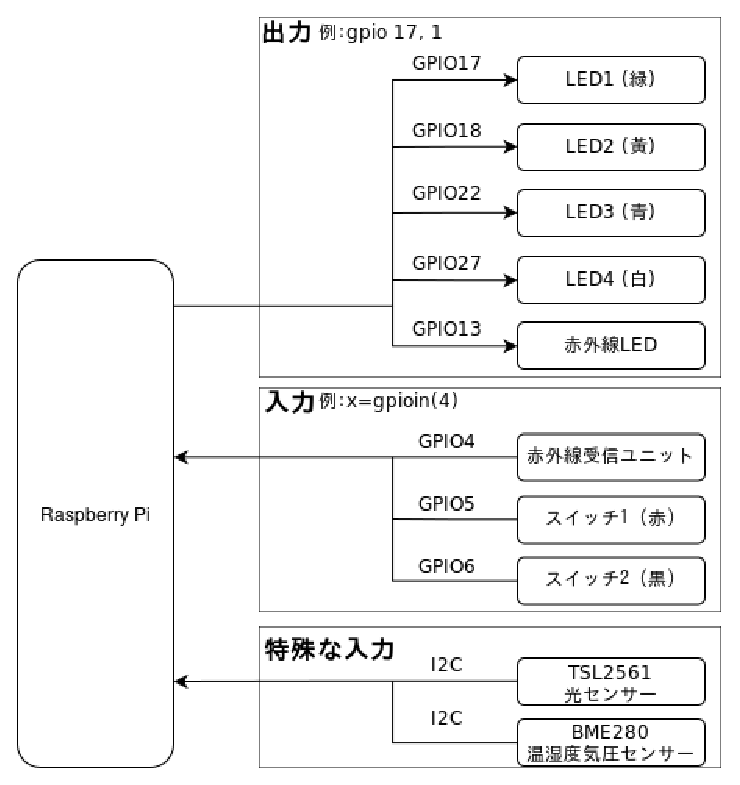
\includegraphics[width=0.6\textwidth]{./text08-img/textbook-img040.eps}

\end{center}


\bigskip


\refstepcounter{Exercise}
\clearpage\section*{\theExercise TV番組表のウェブページをスクレイピングする}
\addtocounter{Exercise}{-1}\refstepcounter{Exercise}\label{E:TV}
考え方

まずは、ウェブブラウザでTV番組表のページを見てみよう。
授業で使用したホームページを開いてください。
\textbf{({\textasciitilde}/08/links.html)}

TV番組表をクリックします。



\begin{center}
  % Unhandled or unsupported graphics:
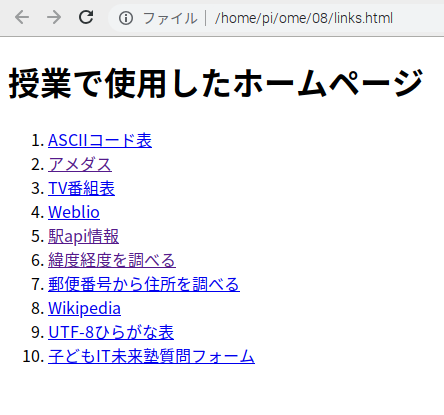
\includegraphics[width=0.6\textwidth]{./text08-img/textbook-img017.png}

\end{center}


\bigskip


TV番組表のウェブページが開きます。
このページの\ruby{検索欄}{けんさくらん}に検索したいワードを入れて検索をすると結果がでてきます。
まずは、\ruby{適当}{てきとう}に検索してみましょう。



\begin{center}
  % Unhandled or unsupported graphics:
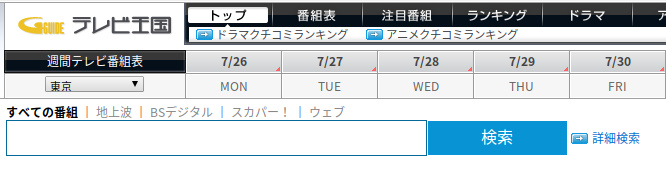
\includegraphics[width=0.85\textwidth]{./text08-img/textbook-img041.png}

\end{center}
\clearpage
試しに”サザエさん”と検索してみました。
結果の画面はこのような感じです。
TVの番組なので検索したタイミングによって番組がやっていなかったりしますのでそのような場合は検索ワードを変更してください。



\begin{center}
  % Unhandled or unsupported graphics:
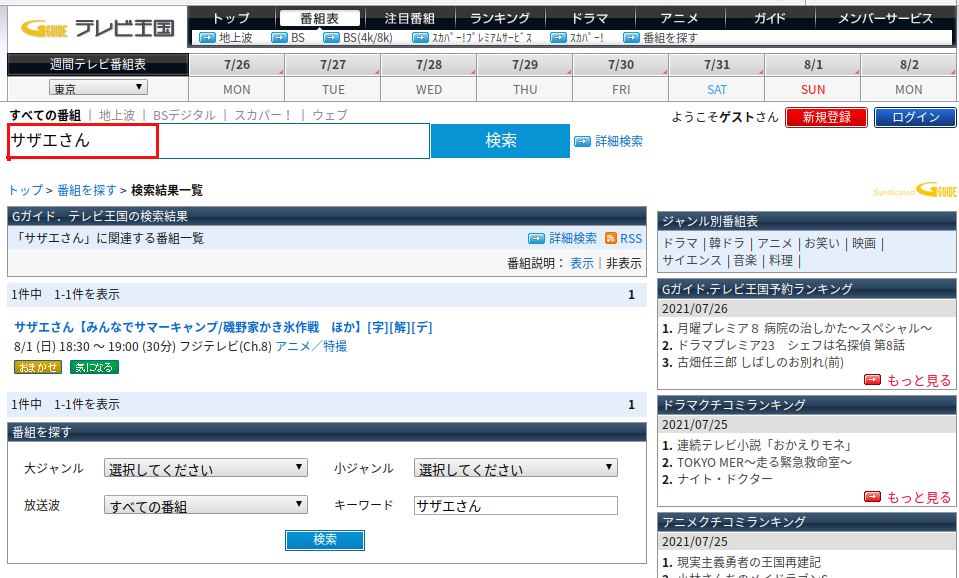
\includegraphics[width=\textwidth]{./text08-img/textbook-img042.png}

\end{center}
今回取得する情報は、検索ワードに対応する検索結果のタイトルと日付です。

まずはプログラムを動かしてみましょう。

ターミナルを開いて

hsed

と実行してスクリプトエディタを開きます。

\begin{center}
  % Unhandled or unsupported graphics:
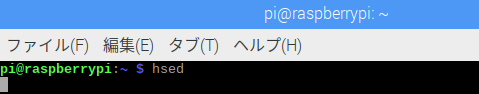
\includegraphics[width=\textwidth]{./text08-img/textbook-img013.png}

\end{center}

\bigskip



\bigskip

\clearpage
HSPスクリプトエディタが開くので

ファイル → 開く..
\ をクリックして\textbf{{\textasciitilde}/08/tv.hsp}を開きます。

プログラムが表示されます。



\begin{center}
  % Unhandled or unsupported graphics:
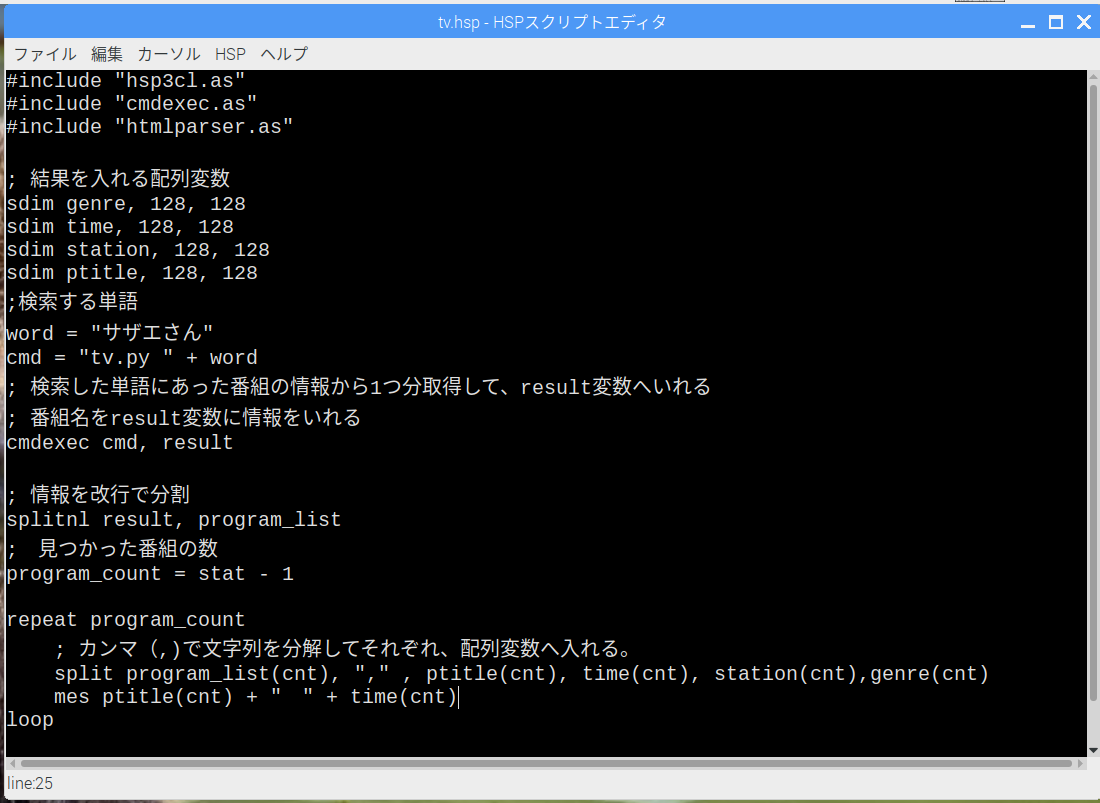
\includegraphics[width=0.85\textwidth]{./text08-img/textbook-img043.png}

\end{center}


\bigskip


F5を押して実行してみましょう。

実行結果はターミナルに表示されます



\begin{center}
  % Unhandled or unsupported graphics:
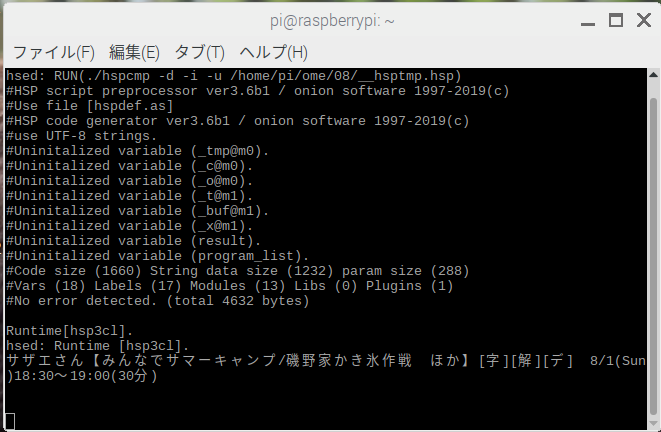
\includegraphics[width=0.85\textwidth]{./text08-img/textbook-img044.png}

\end{center}

\bigskip



ブラウザの表示とプログラムの実行結果を比べてみてください。
実行結果では日付と番組名だけ表示しています

\begin{center}
  % Unhandled or unsupported graphics:
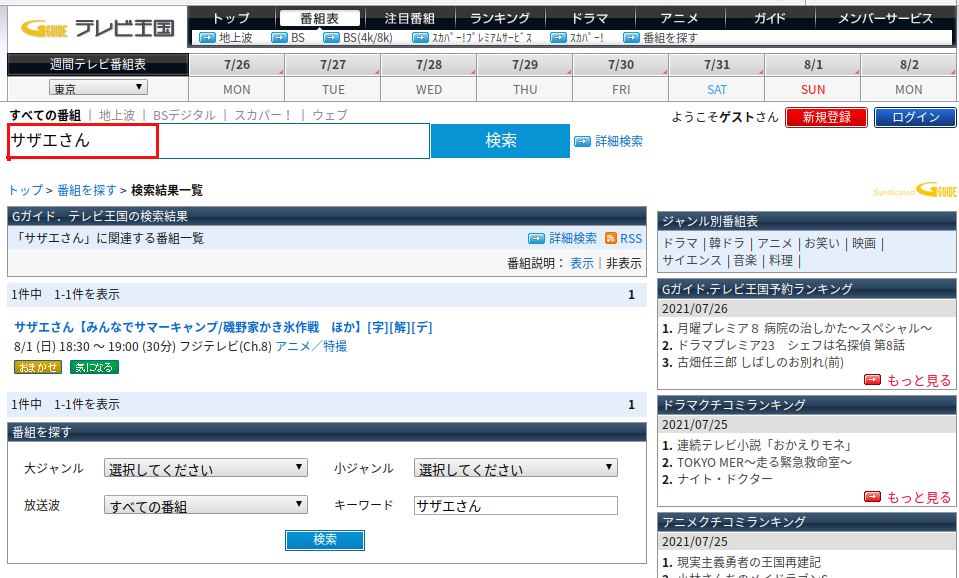
\includegraphics[width=0.85\textwidth]{./text08-img/textbook-img042.png}

\end{center}


\bigskip


\bigskip

\subsection*{}
\refstepcounter{Question}
\subsection*{\theQuestion\label{Q:TV}}
\ \ 6行目のword=”サザエさん”で検索する番組を指定しています。
自分の検索したい番組名にして実行してみましょう。

\refstepcounter{Question}
\subsection*{\theQuestion}
\ \ このプログラムでは、日付(date配列)と番組名(ptitle配列)しか表示をしていません。
ジャンル(genre配列)とテレビ局(station配列)を表示するようにしてみましょう。

\refstepcounter{Exercise}
\clearpage\subsection*{\theExercise Weblioのウェブページをスクレイピングする}
\addtocounter{Exercise}{-1}\refstepcounter{Exercise}\label{E:Weblio}
考え方

まずは、ウェブブラウザでWeblioのページを見てみよう。
授業で使用したホームページを開いてください。
\textbf{({\textasciitilde}/08/links.html)}

Weblioをクリックします。



\begin{center}
  % Unhandled or unsupported graphics:
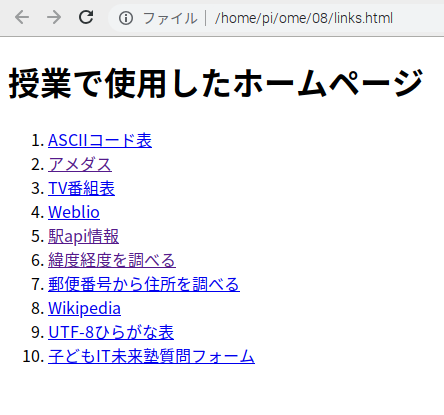
\includegraphics[width=0.5\textwidth]{./text08-img/textbook-img017.png}

\end{center}


Weblioのウェブページが開きます。
このページの検索欄に検索したいワードを入れて検索をすると結果がでてきます。
まずは、適当に検索してみましょう。



\begin{center}
  % Unhandled or unsupported graphics:
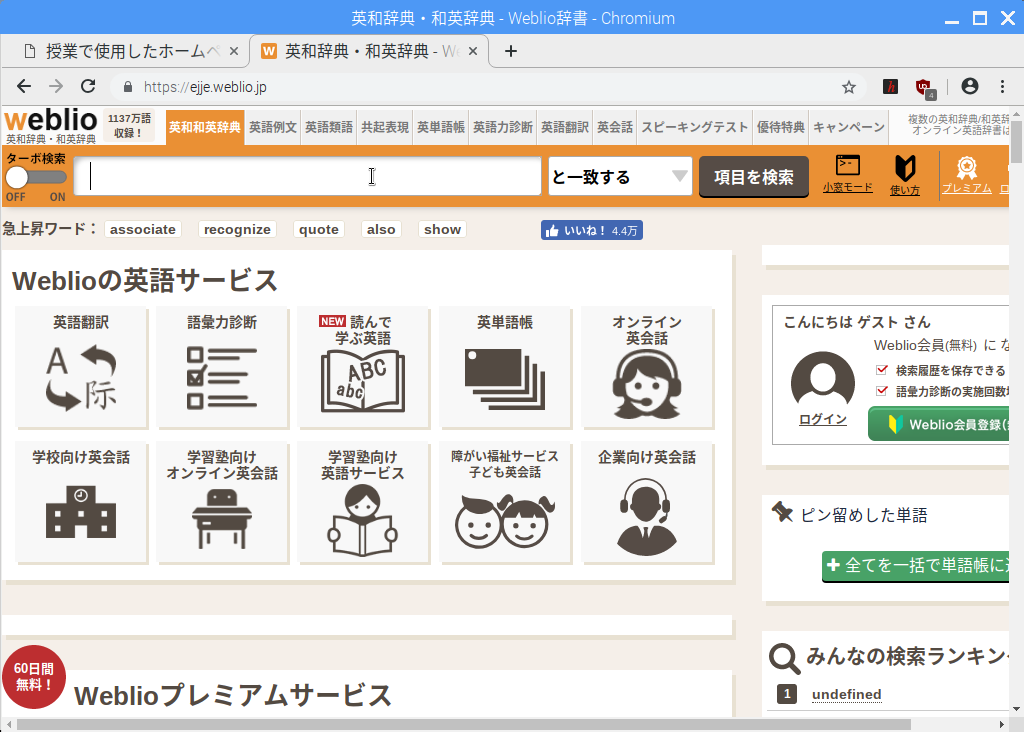
\includegraphics[width=0.8\textwidth]{./text08-img/textbook-img045.png}

\end{center}
\clearpage
試しに”hello”と検索してみました。
結果の画面はこのような感じです。



\begin{center}
  % Unhandled or unsupported graphics:
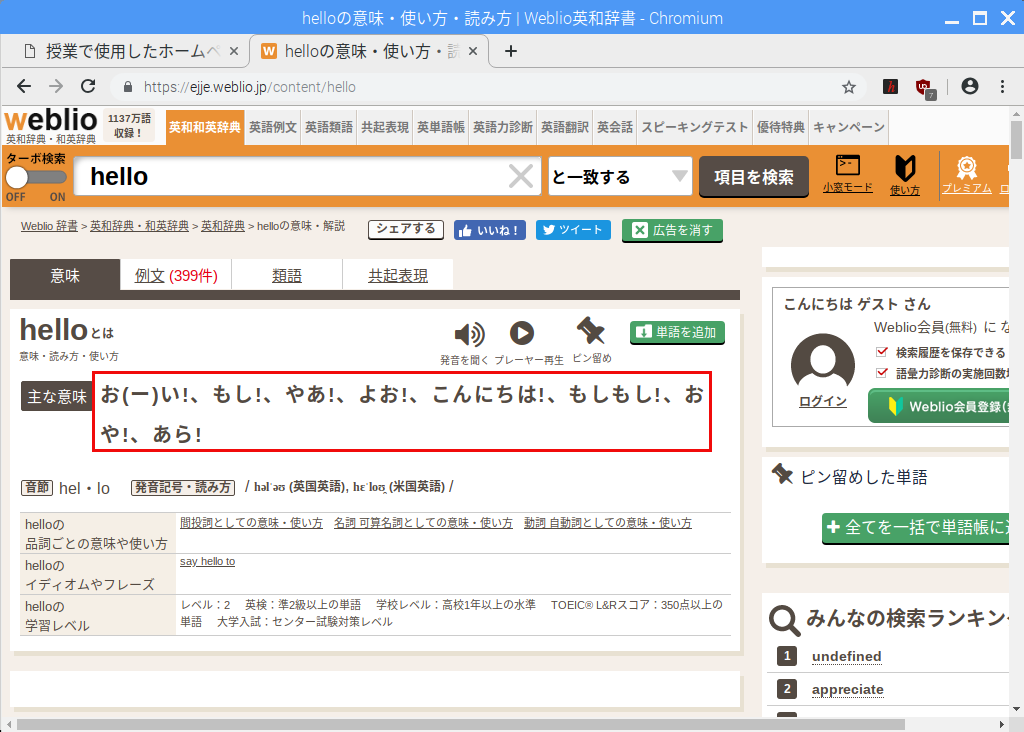
\includegraphics[width=0.8\textwidth]{./text08-img/textbook-img046.png}

\end{center}
今回取得する情報は、検索ワードに対応する主な意味です。

まずはプログラムを動かしてみましょう。

ターミナルを開いて

hsed

と実行してスクリプトエディタを開きます。



\begin{center}
  % Unhandled or unsupported graphics:
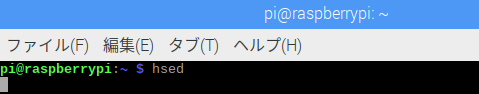
\includegraphics[width=0.9\textwidth]{./text08-img/textbook-img013.png}

\end{center}
\clearpage
HSPスクリプトエディタが開くので

ファイル → 開く..
\ をクリックして\textbf{{\textasciitilde}/08/weblio.hsp}を開きます。

プログラムが表示されます。



\begin{center}
  % Unhandled or unsupported graphics:
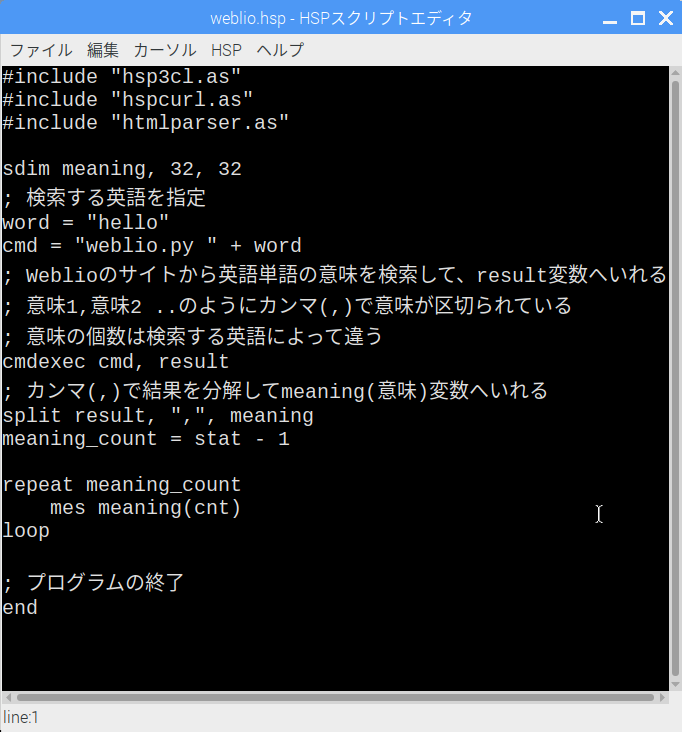
\includegraphics[width=0.7\textwidth]{./text08-img/textbook-img047.png}

\end{center}


\bigskip


F5を押して実行してみましょう。

実行結果はターミナルに表示されます



\begin{center}
  % Unhandled or unsupported graphics:
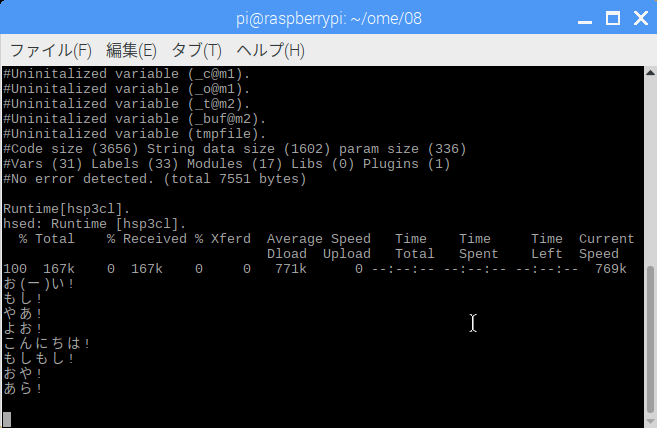
\includegraphics[width=0.7\textwidth]{./text08-img/textbook-img048.png}

\end{center}

\bigskip

\clearpage


ブラウザの表示とプログラムの実行結果を比べてみてください。
”、”で区切られていた意味が表示されています。



\begin{center}
  % Unhandled or unsupported graphics:
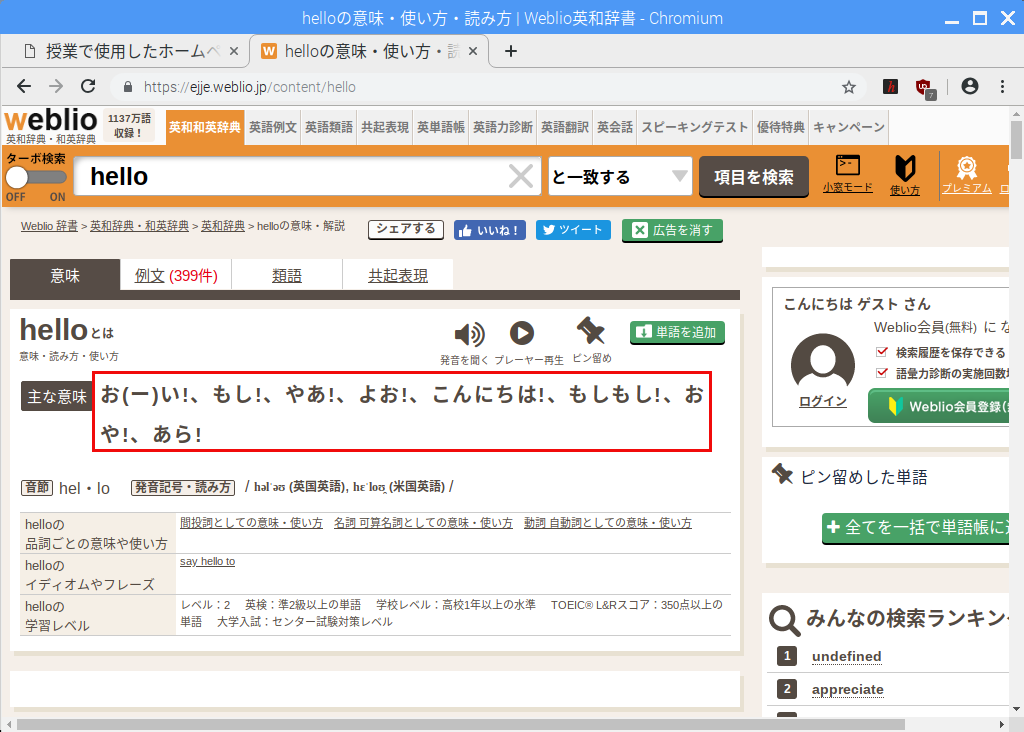
\includegraphics[width=0.9\textwidth]{./text08-img/textbook-img046.png}

\end{center}
\refstepcounter{Question}
\subsection*{\theQuestion\label{Q:weblio}}
7行目のword=”hello”で検索する英語を指定しています。
この変数を自分の検索したい英語にして実行してみましょう。

\ \ HINT : word=”raspberry”


\bigskip

\refstepcounter{Exercise}
\clearpage\subsection*{\theExercise 位置情報のから近くの駅をスクレイピング}
\addtocounter{Exercise}{-1}\refstepcounter{Exercise}\label{E:station}
考え方

まずは、ウェブブラウザで駅検索API情報のページを見てみよう。
授業で使用したホームページを開いてください。
\textbf{({\textasciitilde}/08/links.html)}

駅api情報をクリックします。



\begin{center}
  % Unhandled or unsupported graphics:
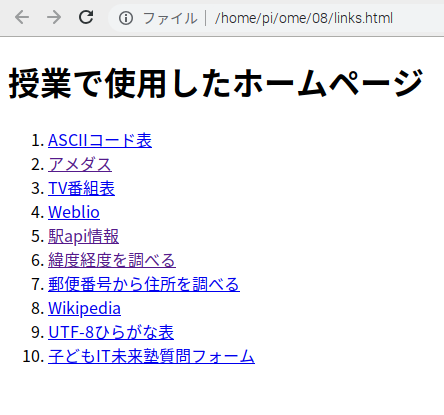
\includegraphics[width=0.5\textwidth]{./text08-img/textbook-img017.png}

\end{center}


駅api情報のウェブページが開きます。
今回使用するのは\ruby{最寄}{もよ}り駅取得 APIです



\begin{center}
  % Unhandled or unsupported graphics:
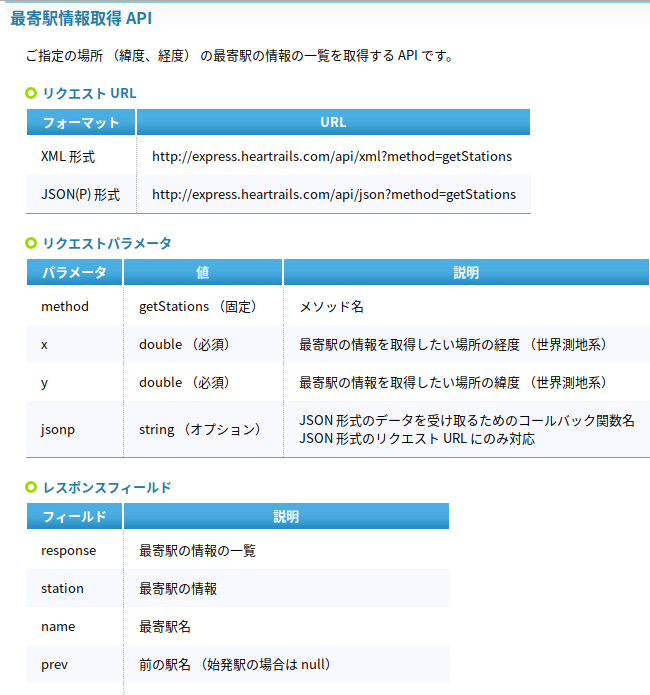
\includegraphics[width=0.6\textwidth]{./text08-img/textbook-img049.png}

\end{center}




\clearpage
まずはプログラムを動かしてみましょう。

ターミナルを開いて

hsed

と実行してスクリプトエディタを開きます。



\begin{center}
  % Unhandled or unsupported graphics:
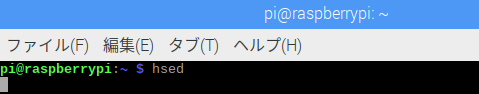
\includegraphics[width=\textwidth]{./text08-img/textbook-img013.png}

\end{center}
HSPスクリプトエディタが開くので

ファイル → 開く..
\ をクリックして\textbf{{\textasciitilde}/08/eki.hsp}を開きます。

プログラムが表示されます。



\begin{center}
  % Unhandled or unsupported graphics:
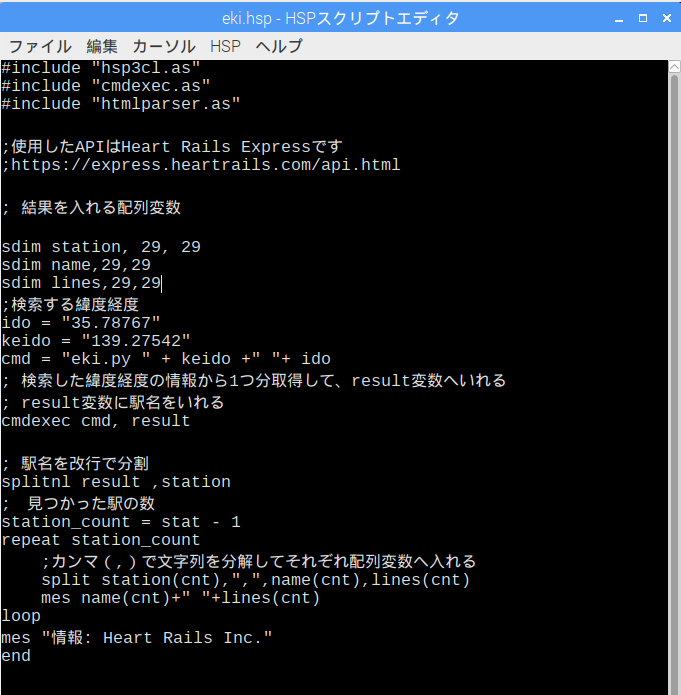
\includegraphics[width=13.377cm]{./text08-img/textbook-img050.png}

\end{center}

\bigskip

\clearpage
F5を押して実行してみましょう。実行結果はターミナルに表示されます



\begin{center}
  % Unhandled or unsupported graphics:
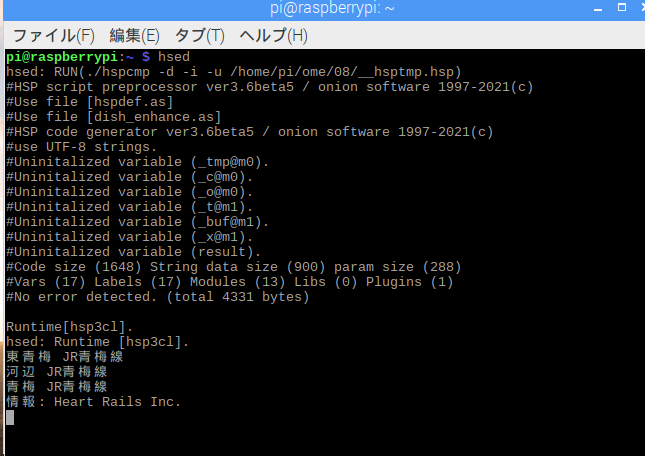
\includegraphics[width=0.8\textwidth]{./text08-img/textbook-img051.png}

\end{center}
ブラウザの表示\\(
\textbf{http://express.heartrails.com/api/xml?method=getStations\&x=139.27542\&y=35.78767}
)とプログラムの実行結果を比べてみてください。
指定した位置に近い駅の名前、その駅の路線名が順に表示されています。



\begin{center}
  % Unhandled or unsupported graphics:
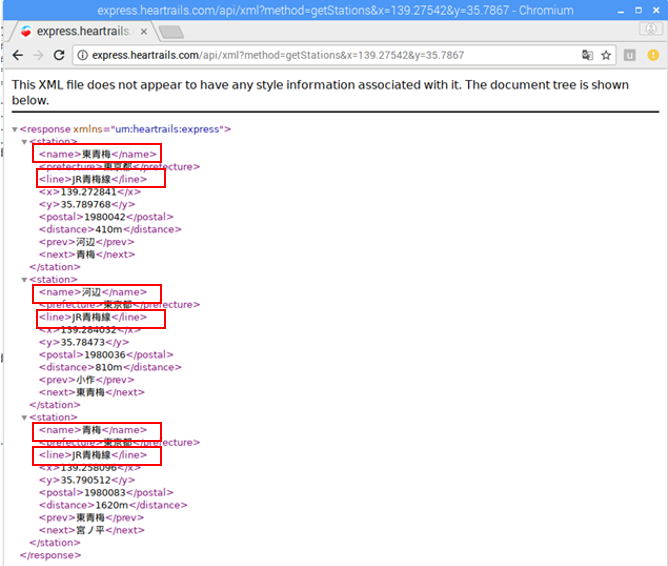
\includegraphics[width=0.8\textwidth]{./text08-img/textbook-img052.png}

\end{center}
\refstepcounter{Question}
\clearpage\subsection*{\theQuestion\label{Q:station}}
\ \ サンプルプログラムでは、青梅市役所の近くの駅名を取得していました。
次は、自分の好きなもしくは知っている場所を指定してみましょう。
\ruby{緯度}{いど}\ruby{経度}{けいど}は、授業で使用したウェブページ\textbf{({\textasciitilde}/08/links.html)}を開いて、

緯度経度を調べるをクリックします。



\begin{center}
  % Unhandled or unsupported graphics:
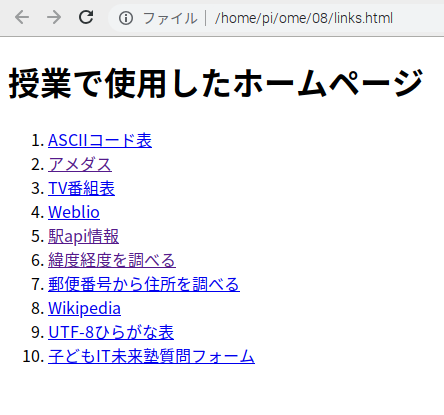
\includegraphics[width=0.5\textwidth]{./text08-img/textbook-img017.png}

\end{center}


フォームで調べたい場所(今回は青梅市役所)を検索(GPS\ruby{座標}{ざひょう}検索)します。



\begin{center}
  % Unhandled or unsupported graphics:
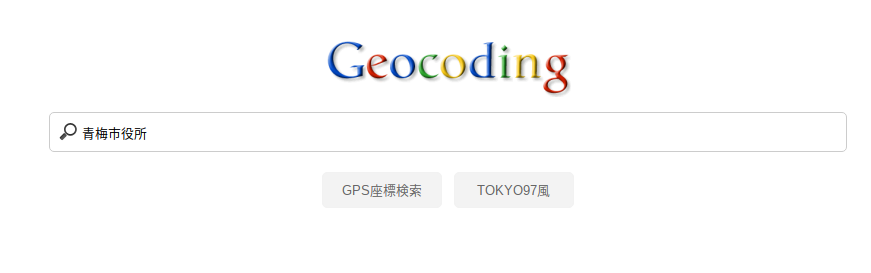
\includegraphics[width=0.8\textwidth]{./text08-img/textbook-img053.png}

\end{center}

\bigskip




\begin{center}
  % Unhandled or unsupported graphics:
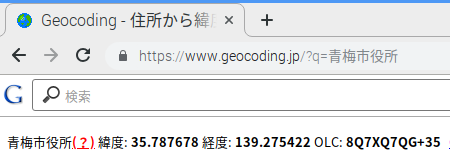
\includegraphics[width=0.5\textwidth]{./text08-img/textbook-img054.png}

\end{center}

\bigskip



検索結果に緯度、経度の数字があります。これをプログラムの



% \begin{center}
% \begin{boxedminipage}{7.959cm}
% Ido=”35.78767”

% keido=”139.27542”
% \end{boxedminipage}
% \end{center}


\begin{table}[htbp]
    \centering
    % \caption{文字タイプ表}
    \begin{tabular}{|l|}
        \hline
        
        Ido=”35.78767”\\
        keido=”139.27542”\\
        \hline
    \end{tabular}
\end{table}


\bigskip


とすると青梅市役所の最寄りの駅とその路線情報を取得して表示することができます。


\bigskip

\refstepcounter{Exercise}
\clearpage\subsection*{\theExercise \ruby{郵便}{ゆうびん}番号から住所を調べるウェブページのスクレイピング}
\addtocounter{Exercise}{-1}\refstepcounter{Exercise}\label{E:postNum}
考え方

まずは、ウェブブラウザで郵便番号から住所を調べるウェブページを見てみよう。
授業で使用したホームページを開いてください。
\textbf{({\textasciitilde}/08/links.html)}

郵便番号から住所を調べるをクリックします。




\begin{center}
  % Unhandled or unsupported graphics:
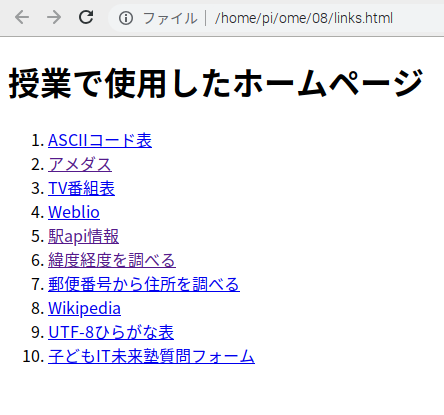
\includegraphics[width=7.181cm]{./text08-img/textbook-img017.png}

\end{center}

\bigskip


\bigskip

郵便番号から住所を調べるウェブページが開きます。
郵便番号に対応する住所ががHTMLのようなページで表示されます。

今回取得する情報は都道府県、市町村です。



\begin{center}
  % Unhandled or unsupported graphics:
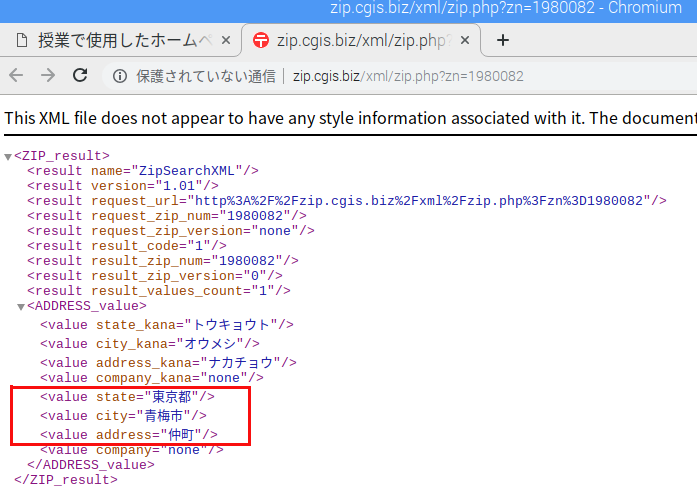
\includegraphics[width=15.492cm]{./text08-img/textbook-img055.png}

\end{center}
\clearpage
まずはプログラムを動かしてみましょう。

ターミナルを開いて

hsed

と実行してスクリプトエディタを開きます。



\begin{center}
  % Unhandled or unsupported graphics:
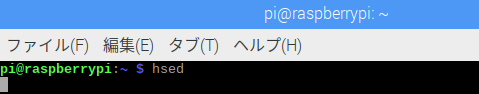
\includegraphics[width=\textwidth]{./text08-img/textbook-img013.png}

\end{center}
HSPスクリプトエディタが開くので

ファイル → 開く..
\ をクリックして\textbf{{\textasciitilde}/08/zipcode.hsp}を開きます。

プログラムが表示されます。



\begin{center}
  % Unhandled or unsupported graphics:
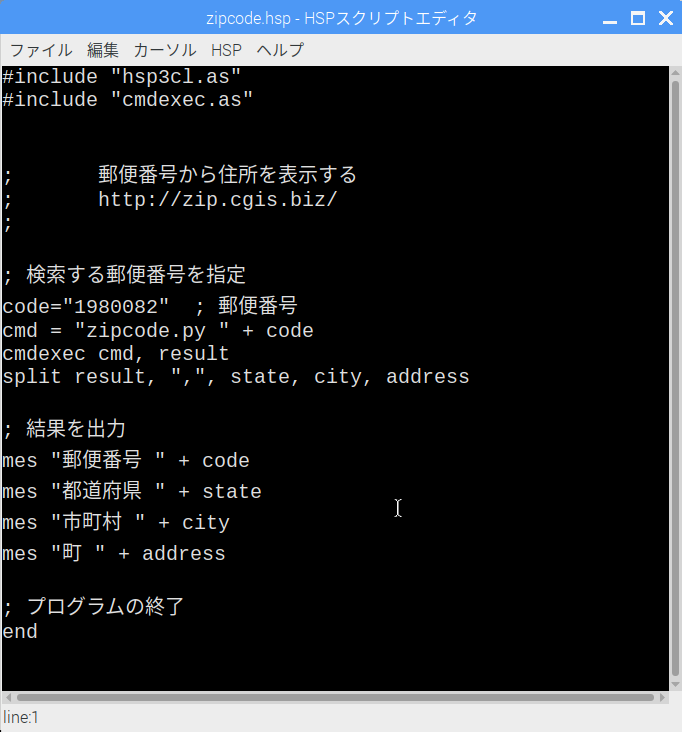
\includegraphics[width=13.951cm]{./text08-img/textbook-img056.png}

\end{center}

\bigskip

\clearpage
F5を押して実行してみましょう。実行結果はターミナルに表示されます



\begin{center}
  % Unhandled or unsupported graphics:
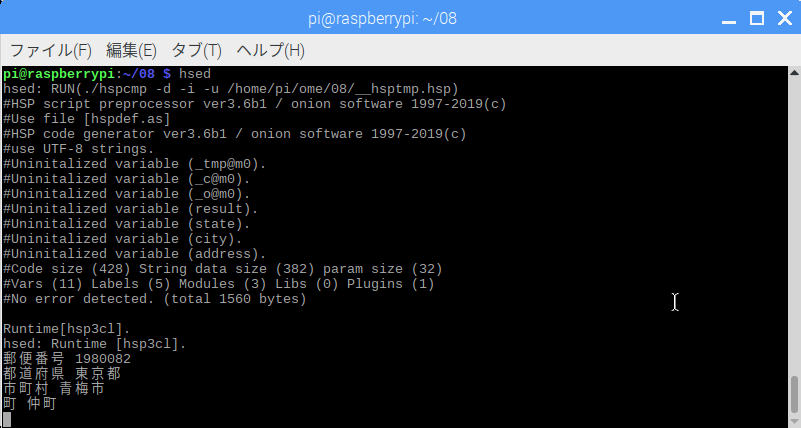
\includegraphics[width=0.8\textwidth]{./text08-img/textbook-img057.png}

\end{center}
ブラウザの表示とプログラムの実行結果を比べてみてください。
郵便番号に対応する都道府県、市町村が表示されているのがわかります。



\begin{center}
  % Unhandled or unsupported graphics:
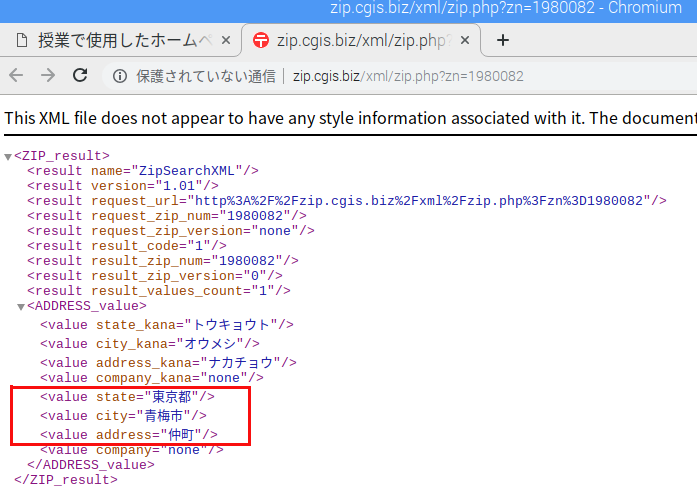
\includegraphics[width=0.8\textwidth]{./text08-img/textbook-img055.png}

\end{center}



\refstepcounter{Question}
\subsection*{\theQuestion\label{Q:postNum}}
\ \ codeの郵便番号を変更してみよう

\ \ 例: 198-0082
青梅\ruby{佐藤財団}{さとうざいだん}の郵便番号

% \begin{center}
% \begin{boxedminipage}{10.927cm}
% \begin{enumerate}
% \item code = “1980082”
% \end{enumerate}
% \end{boxedminipage}
% \end{center}


\begin{table}[htbp]
    \centering
    % \caption{文字タイプ表}
    \begin{tabular}{|l|}
        \hline
        
        1. code = “1980082” \\
        \hline
    \end{tabular}
\end{table}




\refstepcounter{Exercise}
\clearpage\subsection*{\theExercise Wikipediaのスクレイピング}
\addtocounter{Exercise}{-1}\refstepcounter{Exercise}\label{E:wikipedia}
考え方

まずは、ウェブブラウザでWikipediaを見てみよう。
授業で使用したホームページを開いてください。
\textbf{({\textasciitilde}/08/links.html)}

Wikipediaをクリックします。



\begin{center}
  % Unhandled or unsupported graphics:
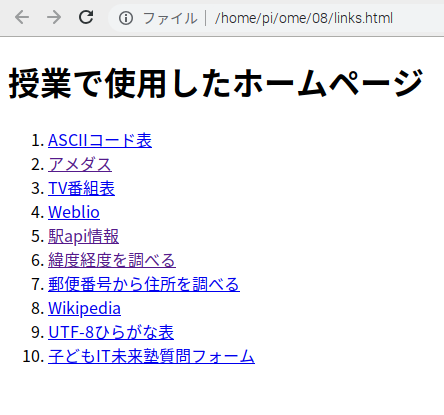
\includegraphics[width=0.5\textwidth]{./text08-img/textbook-img017.png}

\end{center}


Wikipediaが開きます。
このページの検索欄に検索したいワードを入れて検索をすると結果がでてきます。
まずは、適当に検索してみましょう。



\begin{center}
  % Unhandled or unsupported graphics:
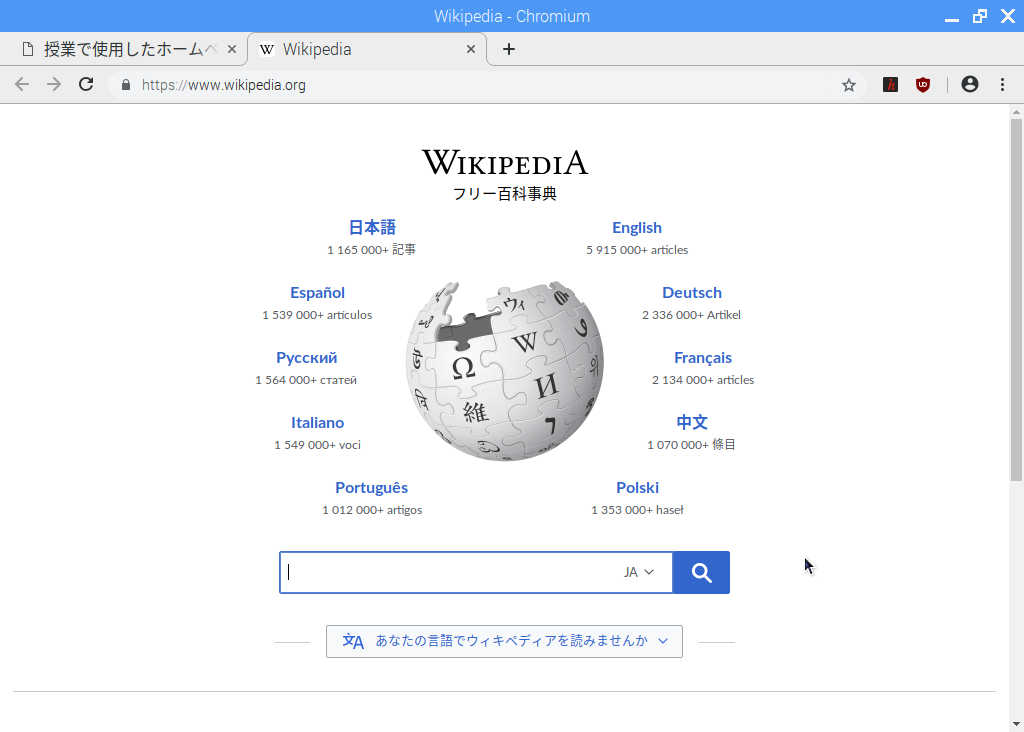
\includegraphics[width=0.8\textwidth]{./text08-img/textbook-img058.png}

\end{center}
\clearpage
試しに”Raspberry
Pi”と検索してみました。
結果の画面はこのような感じです。



\begin{center}
  % Unhandled or unsupported graphics:
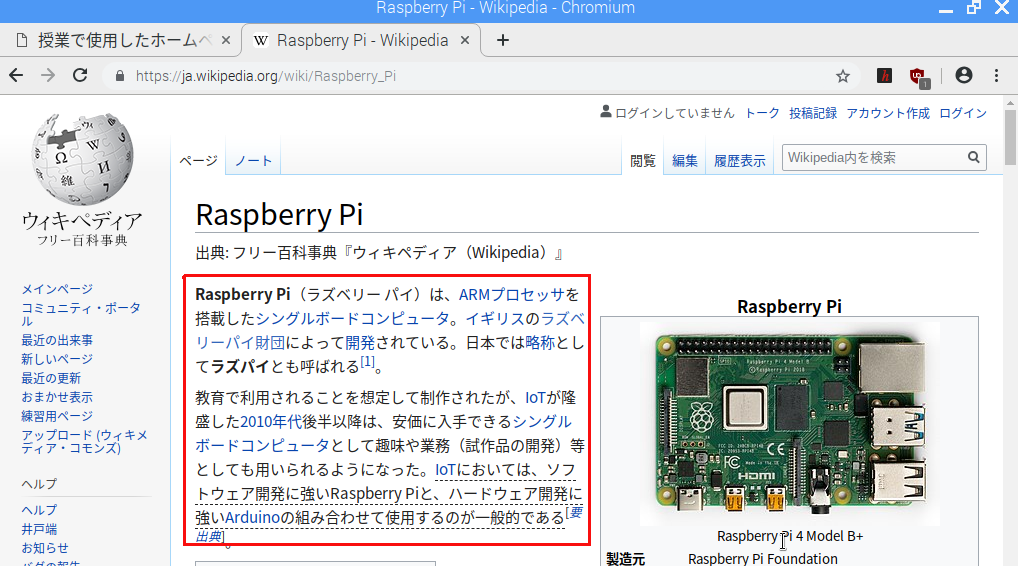
\includegraphics[width=0.9\textwidth]{./text08-img/textbook-img059.png}

\end{center}
今回取得する情報はラズベリーパイの\ruby{概要}{がいよう}です。

まずはプログラムを動かしてみましょう。

ターミナルを開いて

hsed

と実行してスクリプトエディタを開きます。



\begin{center}
  % Unhandled or unsupported graphics:
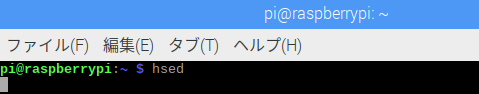
\includegraphics[width=0.9\textwidth]{./text08-img/textbook-img013.png}

\end{center}

\bigskip

\clearpage
HSPスクリプトエディタが開くので


\bigskip

ファイル → 開く..
\ をクリックして\textbf{{\textasciitilde}/08/wikipedia.hsp}を開きます。

プログラムが表示されます。



\begin{center}
  % Unhandled or unsupported graphics:
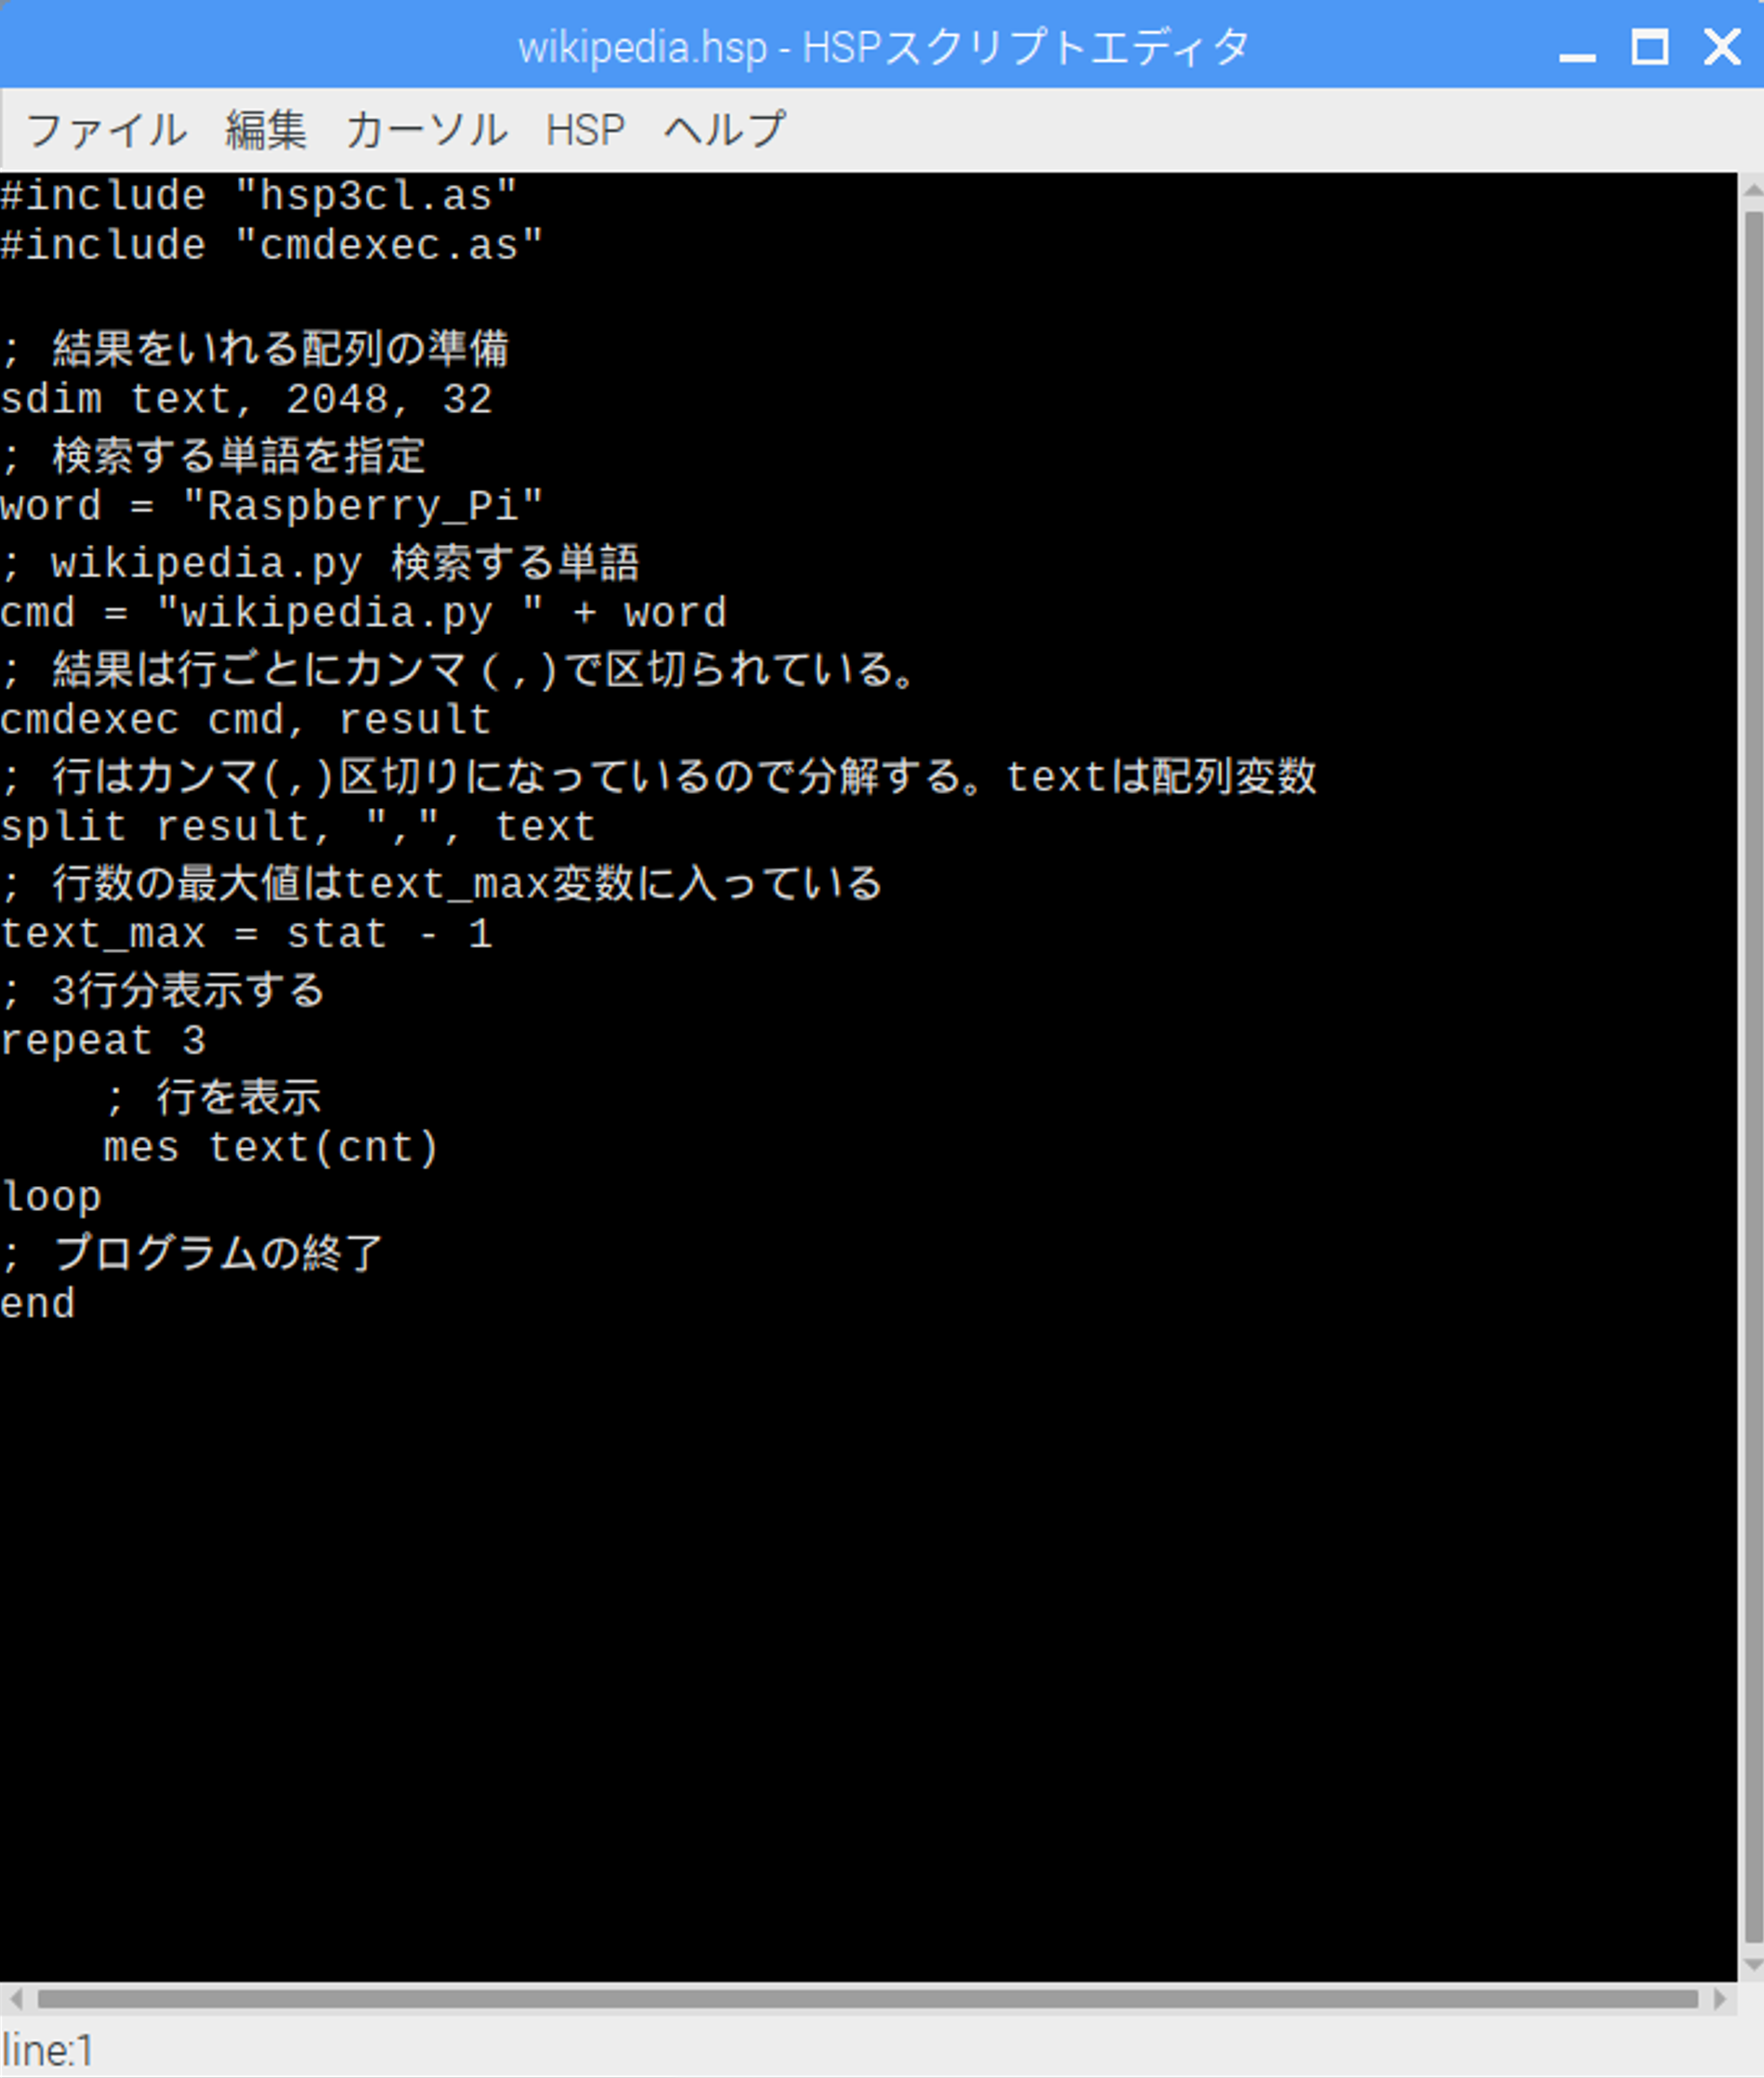
\includegraphics[width=\textwidth]{./text08-img/img00060.png}

\end{center}

\bigskip

\clearpage
F5を押して実行してみましょう。実行結果はターミナルに表示されます



\begin{center}
  % Unhandled or unsupported graphics:
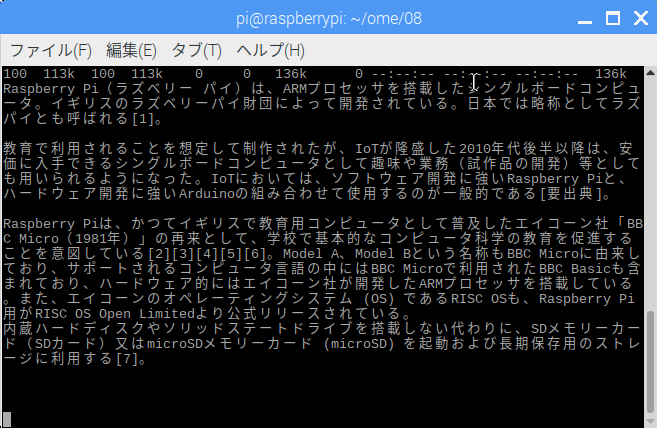
\includegraphics[width=\textwidth]{./text08-img/textbook-img061.png}

\end{center}
ブラウザの表示とプログラムの実行結果を比べてみてください。
検索用語(Raspberry
Pi)の概要がWikipediaからとれました。



\begin{center}
  % Unhandled or unsupported graphics:
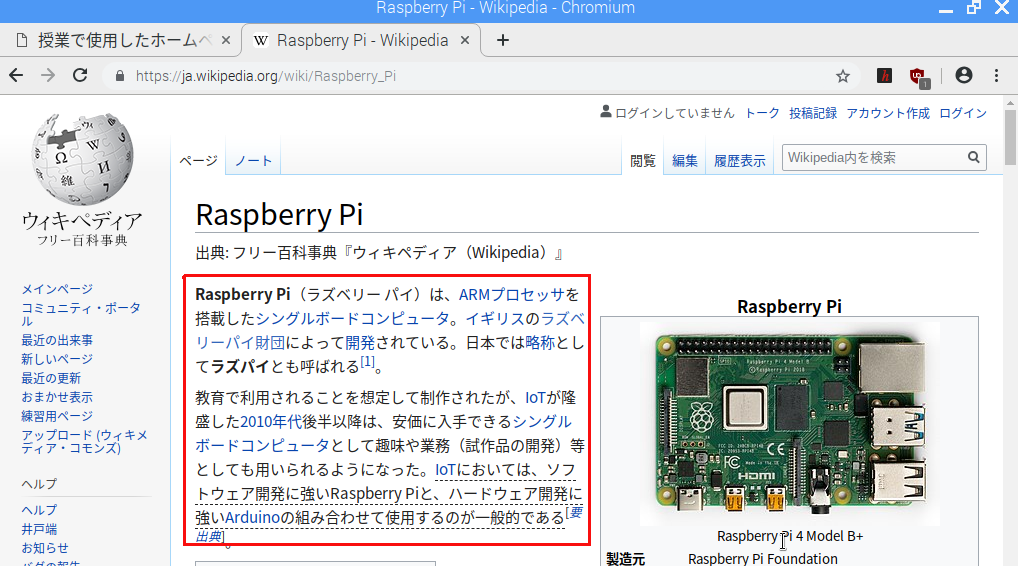
\includegraphics[width=\textwidth]{./text08-img/textbook-img059.png}

\end{center}

\bigskip

\refstepcounter{Question}
\subsection*{\theQuestion\label{Q:wikipedia}}
wordを自分の検索したい単語に変えてみよう。

\ \ HINT:まずは、Wikipediaで検索したい単語を検索をしてみて、ページを開きましょう。

URLの

http://ja.wikipedia.org/wiki/*******

wiki/より後にある文字列をwordに入れます。



\begin{center}
  % Unhandled or unsupported graphics:
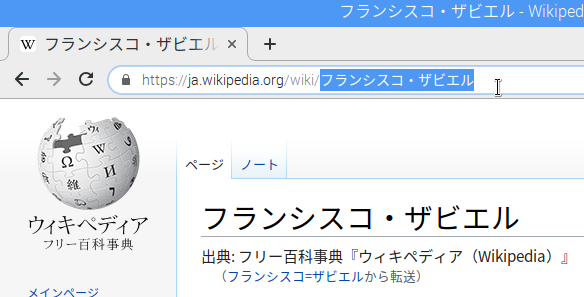
\includegraphics[width=0.9\textwidth]{./text08-img/textbook-img062.png}

\end{center}
例えば、

word = “フランシスコ・ザビエル”

検索用語によってはページがWikipediaにないことがあります。
